\documentclass[aspectratio=43]{beamer}

\usepackage[utf8]{inputenc} % mindenképp maradjon az utf-8 kódolás
\usepackage[magyar]{babel}
\usepackage[T1]{fontenc}
\usepackage{amsmath}
\usepackage{amsfonts}
\usepackage{amssymb}
\usepackage{graphicx} % grafikus elemek, képek berakásához
%\usepackage{blindtext}
%\usepackage{hyperref} % PDF hivatkozásokhoz kell
\usepackage[hang]{caption}
%\usepackage{xcolor}
%\usepackage[affil-it]{authblk}

%\definecolor{rosewood}{rgb}{0.6, 0.0, 0.04}
%\definecolor{indigo(dye)}{rgb}{0.0, 0.25, 0.42}

\usetheme{default}	% téma
\usecolortheme{seahorse}
\usefonttheme{serif}	% gyönyörű talpas betűtípus

\beamertemplatenavigationsymbolsempty % a pdf-be ágyazott navigációs gombok kikapcsolása

\title{Modell-redukció alkalmazása\\az elektromágneses térszámításban}			% cím
%\subtitle{\vspace{0.3cm}Proper Orthogonal Decomposition} 	% alcím

\date{\today}

\author{Szilágyi Gábor\\[3ex]Konzulens: Dr. Bilicz Sándor}	% szerző

%\institute{Institute} % intézmény vagy más infó a szerzőről
%\logo{
\includegraphics[height=0.5cm]{bme_logo.pdf}}
%\newcommand{\pagenum}{\hfill\insertframenumber/\insertpresentationendpage\hspace{-\fill}}
\newcommand{\numframetitle}[1]{\frametitle{#1\hfill\insertframenumber/\insertpresentationendpage\hspace{-\fill}}}
\begin{document}
\maketitle	% címoldal
\begin{frame}
	\numframetitle{A nagy szabadsági fok problémája}
	\begin{columns}
		\column{0.48\textwidth}
            \begin{center}
    		    Bonyolult szimulálandó modell
                \begin{align*}
                    \Downarrow
                \end{align*}
                Sok szabadsági fok
                \begin{align*}
                    \Downarrow
                \end{align*}
            \end{center}
            \begin{itemize}
                \item Nagy egyenletrendszer
                \item Sok ($n$) ismeretlen
                \item Nagy memóriaigény
                \item Hosszú számítási idő
            \end{itemize}
        \column{0.48\textwidth}
	        Sokszor nem megengedhető az egyszerűbb modell\\[3ex]
            (pl. ritkább végeselem háló)\\[3ex]
            $n$ nem csökkenthető
    \end{columns}
\end{frame}
\begin{frame}
	\numframetitle{Modell-redukció}
    \framesubtitle{POD (Proper Orthogonal Decomposition)}
	\begin{columns}
		\column{0.48\textwidth}
            A bonyolult modell megoldását közelítjük kevesebb ($r< n$) szabadsági fokkal\\[3ex]
            Közelítő, olcsó megoldás a bonyolult problémára\\[3ex]
            Kisebb egyenletrendszert kell megoldani ($r$ egyenlet), de mind az $n$ ismeretlenre lesz közelítő eredmény
		\column{0.48\textwidth}
            POD:\\[3ex]
            \begin{center}
                $\mathbf{X}$ Adathalmaz
                \begin{align*}
                    \Downarrow
                \end{align*}
                Csonkításhoz optimális\\ sorbarendezett $\Psi$ bázis\\[1ex] \large\underline{$\mathbf{X}$-hez}\normalsize
            \end{center}
            \begin{align*}
                \Psi &= \left\{ \Psi_1,\,\Psi_2,\,...\,,\,\Psi_n\right\}\\
                \Psi' &= \left\{ \Psi_1,\,\Psi_2,\,...\,,\,\Psi_r\right\}
            \end{align*}
	\end{columns}
\end{frame}
\begin{frame}
	\numframetitle{Honnan jön \textbf{X}? Hol használjuk fel?}
    	\begin{figure}
			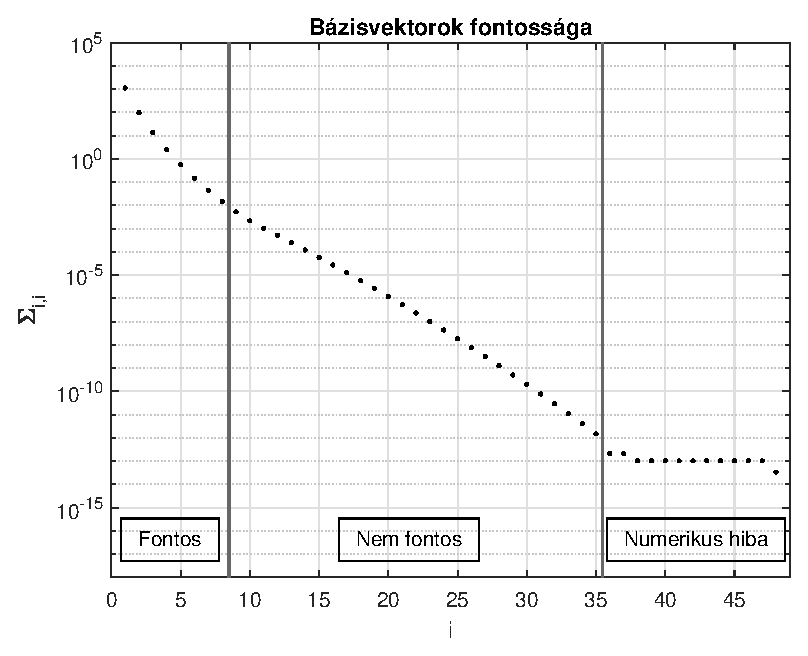
\includegraphics[width=0.7\textwidth]{kep/euler_0.15_4_sv.eps}
		\end{figure}
\end{frame}
\begin{frame}
	\numframetitle{POD algoritmus: SVD}
    \framesubtitle{Singular Value Decomposition}
    	\begin{figure}
			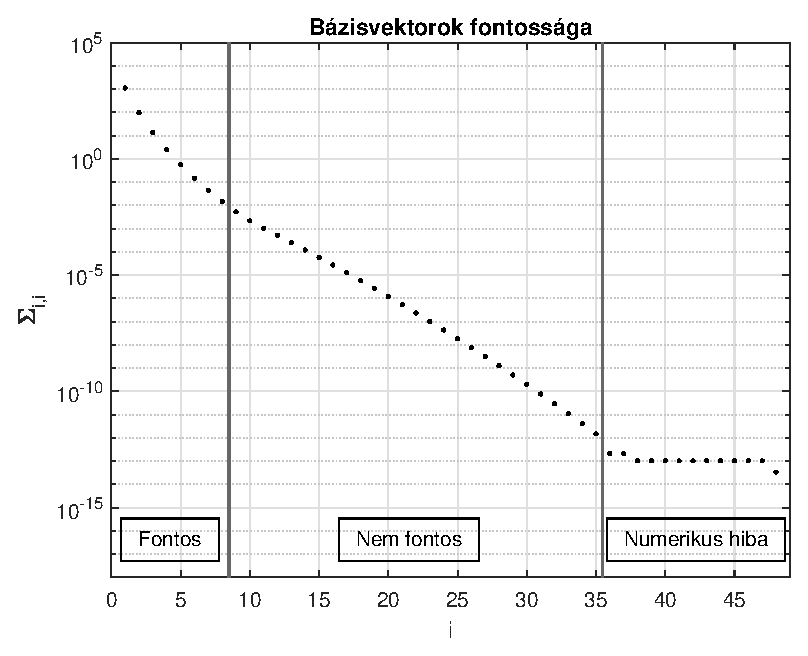
\includegraphics[width=0.7\textwidth]{kep/euler_0.15_4_sv.eps}
		\end{figure}
\end{frame}
\begin{frame}
	\numframetitle{Csonkításból adódó hiba}
    	\begin{figure}
			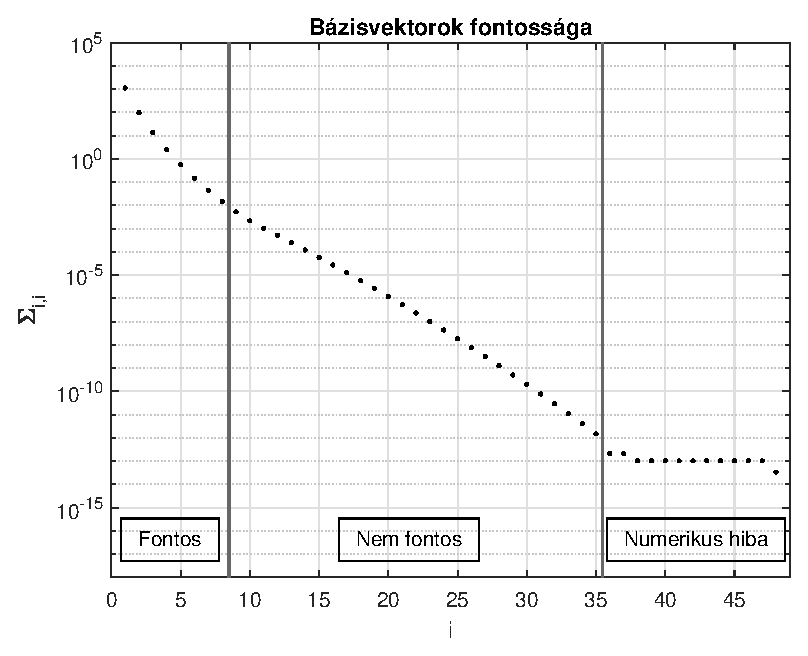
\includegraphics[width=0.7\textwidth]{kep/euler_0.15_4_sv.eps}
		\end{figure}
\end{frame}
\end{document}
